%This chapter describes a collection of projects comprising the \textit{Neuro-Episodic Schema Learner} (NESL). \footnote{Spoken aloud, ``NESL'' shares its pronounciation with the English word \textit{nestle}.} In the previous chapter, I discussed the fundamental approach to EL schema acquisition: beginning with protoschemas, taxonomic specifications of known schemas are acquired via matching with text and composed into more complex schemas; these complex schemas are then stored and potentially generalized with other, similar schemas to focus on salient details at a reasonable level of generality. NESL is intended as an initial implementation of that general approach to schema learning; designed as a pipeline that incorporates pre-trained, state-of-the-art models, NESL leverages the flexibility of neural representation to match an initial set of protoschemas to text, and to learn coherent event schemas that exclude overly specific details.



%%%%%

\begin{figure}
    \centering
    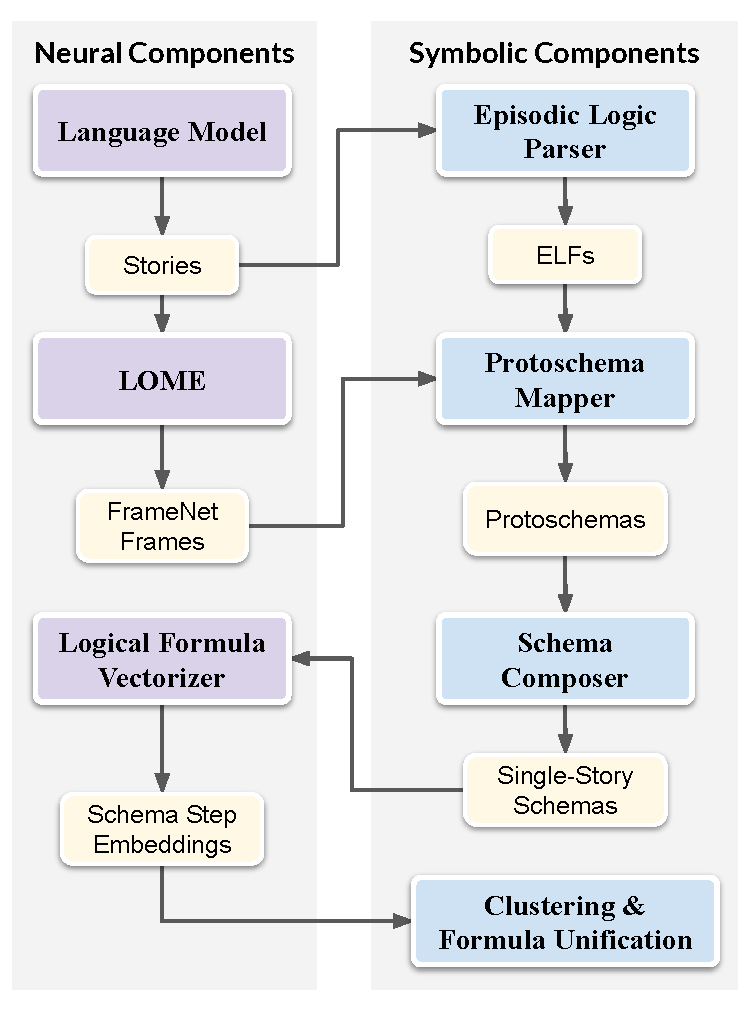
\includegraphics[]{figures/nesl/srw_architecture}
    \caption{A diagram of the NESL schema learning pipeline. NESL makes extensive use of both \textit{neural} and \textit{symbolic} components to acquire event schemas from GPT-J 6B, a large language model.}
    \label{fig:nesl_architecture}
\end{figure}

Work on the task of event schema acquisition is largely separable into two main camps: the \textit{symbolic} camp, with its structurally rich but infamously brittle representations \citep{lebowitz1980,norvig1987inference,mooney1990general}; and the \textit{statistical} camp, which utilizes complex models and vast amounts of data to produce large numbers of conceptually varied event schemas at the cost of representational richness and control over what schemas are learned \citep{chambers2008unsupervised,pichotta2016learning,wanzare2017inducing}. In an attempt to bridge these camps together, this chapter introduces the Neuro-Episodic Schema Learner (NESL)\footnote{Spoken aloud, ``NESL'' shares its pronounciation with the English word \textit{nestle}.}, a composite pipeline model bringing together (1) a large, pre-trained language model; (2) word vector embedding techniques; (3) a neural FrameNet parsing and information extraction system; (4) a formal logical semantic representation of English; and (5) a hierarchical event schema framework with extraordinary expressive power.

In Chapter~\ref{chap:schemas}, I discussed the fundamental approach to EL schema acquisition: beginning with protoschemas, taxonomic specifications of known schemas are acquired via matching with text and composed into more complex schemas; these complex schemas are then stored and potentially generalized with other, similar schemas to focus on salient details at a reasonable level of generality. NESL is intended as an initial implementation of that general approach to schema learning; designed as a pipeline that incorporates pre-trained, state-of-the-art models, NESL leverages the flexibility of neural representation to match an initial set of protoschemas to text, and to learn coherent event schemas that exclude overly specific details.

A key contribution of NESL is the idea of \textit{latent schema sampling} (LSS), in which a pre-trained language model is induced, via prompt-engineering, into acting as a distribution over stories, parameterized by an implicit \textit{latent schema} coarsely established by the prompt. By finding commonalities between multiple samples from this distribution and discarding infrequent details, NESL attempts to generate more accurate, less noisy schemas. In addition to eliminating NESL's need for its own training corpus, LSS allows NESL to generate schemas for user-provided situation descriptions on demand, greatly increasing the control over what sorts of event schemas are generated.

\iffalse
NESL learns schemas using a multi-step pipeline, briefly described in order here, and further expounded upon in following subsections:
\begin{enumerate}
    \item Using a procedure we call \textit{latent schema sampling}, $N$ short stories are sampled from the same topic-parameterized distribution defined by a language model and a task-specific prompt. (Section~\ref{sec:lss})
    \item The $N$ stories are then parsed into Episodic Logical Form (ELF), the formal semantic representation underlying the event schemas.
    \item Simple protoschemas are then matched to each of the $N$ EL-parsed stories with the help of LOME, a state-of-the-art neural FrameNet parser, whose identified FrameNet frames are mapped to corresponding EL protoschemas. (Section~\ref{sec:lome})
    \item For each of the $N$ stories, all identified protoschemas, and all unmatched ELF episodes and type formulas from the story, are composed into a \textit{single-story schema}, in which constants are abstracted to variables and type-constrained, and events are related with a time graph. (Section~\ref{sec:singleschemas})
    \item The $N$ single-story schemas are generalized into a single schema, incorporating common details and excising specious, incidental information from the entire set. (Section~\ref{sec:schemagen})
\end{enumerate}
\fi

In Section~\ref{sec:lome}, I describe NESL's use of a neural FrameNet parser to identify protoschemas in texts and form full EL protoschemas from those texts. In Section~\ref{sec:lss}, I describe and formally define latent schema sampling. Sections~\ref{sec:singleschemas}~and~\ref{sec:schemagen} then respectively describe the processes of forming and generalizing schemas from sampled stories. Finally, in Section~\ref{sec:nesl_discussion}, I discuss NESL's role and contributions in relation to the wider schema learning project, making the case that improving the performance of component parts and widening the scope of initial knowledge types is necessary to learn truly human-like schemas.

%In Section~\ref{sec:lome}, I describe NESL's use of a neural FrameNet parser to identify protoschemas in texts and form full EL protoschemas from those texts. Then, in Section~\ref{sec:nesl}, I describe the full NESL pipeline, including the \textit{latent schema sampling} (LSS) algorithm underlying the approach.


%The remainder of this paper is organized into a description of our chosen semantic representation and event schema framework (Section~\ref{sec:schemarep}); a description of each of NESL's components (Section~\ref{sec:pipeline}); and a description of future evaluation work we intend to complete in the near future (Section~\ref{sec:eval}).